\textbf{ACC to write the first version}


The access control for the SPHR is handled by Smart Contracts running on Blockchain. The following is the process flow:

\begin{enumerate}
    \item The Hospital (organisation) creates generic access rules about its data, these rules are written in the Blockchain
    \item The Patient creates access rules about this data, these rules are written in the Blockchain
    \item Identifier of the Patient is shared with the data requester
    \item The Doctor authenticates himself
    \item The Doctor (Individual, belonging to a group in an organisation) requests access to data about a Patient (from a Hospital). The Doctor identifier and the Patient identifier are checked against the access rules in the Blockchain (Check/Audit trail)
    \item An access token (or decryption key) is requested from the data vault to access the Patient data
    \item The data vault provides the access token (or decryption key)
    \item A response is sent to the Doctor with access token (or decryption key)
    \item The Doctor requests data about the Patient to the data vault using his access token (or decryption key)
    \item The data vault provides the requested data 
\end{enumerate}

\begin{figure}[H]
    \centering
    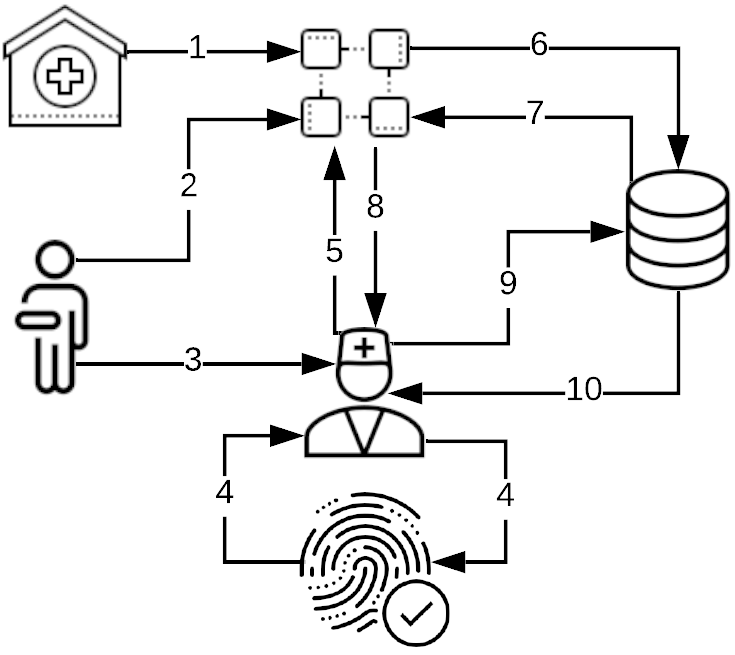
\includegraphics[width=70mm]{images/DataVault/blockchain.png}
    \caption{Process flow for access request}
    \label{fig:blockchain_flow}
\end{figure}



\textbf{ACC to write the first version}


% Need write-up of smart contracts and block chain